
%(BEGIN_QUESTION)
% Copyright 2010, Tony R. Kuphaldt, released under the Creative Commons Attribution License (v 1.0)
% This means you may do almost anything with this work of mine, so long as you give me proper credit

When ``locking out'' a complex piece of equipment or machinery for maintenance work, a large number of different energy-flow devices (e.g. circuit breakers, block valves, bleed valves) must be secured in their safe positions by multiple workers.  If each worker were to place their own personal padlock on each of these devices, the total number of locks required would be staggering.

A more efficient system for managing this is to use a sheet-metal box containing a numbered padlock (with matching key) for each energy-flow device to be secured on the equipment, as well as a list identifying which lock goes on which energy-flow device.  The lid of this device is then lock-able with a multi-lock device, permitting multiple peoples' personal locks to be applied so the lid cannot be opened unless {\it all} personal locks are removed from it:

$$\includegraphics[width=15.5cm]{i01858x01.eps}$$

Explain how having numbered padlocks stored inside this lock-box prior to a job, and by having workers apply their personal padlocks to secure the lid of this lock-box, help to ensure the equipment will be safe for everyone to work on.  

Also, identify any way(s) this safety system could fail, thereby placing people in danger.

\vskip 50pt

\underbar{file i01858}
%(END_QUESTION)





%(BEGIN_ANSWER)


%(END_ANSWER)





%(BEGIN_NOTES)

Critical points to include:

\begin{itemize}
\item{} Locate sources of potentially hazardous energy and how to secure them.
\item{} Secure all valves and electrical disconnects, then safety-tag and lock it in the safe position.
\item{} Test the equipment to ensure the energy source has been secured.
\end{itemize}

The safety tag should describe who is working on the equipment, the date of tagging, the nature of the work, and the expected duration.  Locks should be keyed such that no one can open a lock for someone else (e.g. a personal lock, and not a shop lock).

%INDEX% Safety, lock-out / tag-out: community lock-box

%(END_NOTES)


